\documentclass[notes,11pt, aspectratio=169]{beamer}

\usepackage{pgfpages}
\setbeameroption{hide notes} % Only slide

\usepackage{array}
\usepackage{tikz}
\usepackage{verbatim}
\setbeamertemplate{note page}{\pagecolor{gray!5}\insertnote}
\usetikzlibrary{positioning}
\usetikzlibrary{snakes}
\usetikzlibrary{calc}
\usetikzlibrary{arrows}
\usetikzlibrary{decorations.markings}
\usetikzlibrary{shapes.misc}
\usetikzlibrary{matrix,shapes,arrows,fit,tikzmark}
\usepackage{amsmath}
\usepackage{mathpazo}
\usepackage{hyperref}
\usepackage{lipsum}
\usepackage{multimedia}
\usepackage{graphicx}
\usepackage{multirow}
\usepackage{dcolumn}
\usepackage{bbm}
\newcolumntype{d}[0]{D{.}{.}{5}}

\usepackage{changepage}
\usepackage{appendixnumberbeamer}

\usepackage[space]{grffile}
\usepackage{booktabs}

% Colors
\definecolor{blue}{RGB}{0,114,178}
\definecolor{red}{RGB}{213,94,0}
\definecolor{yellow}{RGB}{240,228,66}
\definecolor{green}{RGB}{0,158,115}
\definecolor{solutionbg}{RGB}{240,248,240}
\definecolor{solutionframe}{RGB}{0,158,115}

% Solution box environment for worked answers
\usepackage{tcolorbox}
\newtcolorbox{solutionbox}[1][]{
  enhanced,
  colback=solutionbg,
  colframe=solutionframe,
  boxrule=0pt,
  leftrule=3pt,
  arc=0pt,
  left=8pt,
  right=8pt,
  top=6pt,
  bottom=6pt,
  fonttitle=\bfseries,
  title={#1},
  attach boxed title to top left={yshift=-2mm, xshift=5mm},
  boxed title style={colback=solutionframe, colframe=solutionframe, size=small, arc=2pt}
}

\hypersetup{
  colorlinks=false,
  linkbordercolor = {white},
  linkcolor = {blue}
}

\definecolor{MyBackground}{RGB}{255,253,218}

\newenvironment{transitionframe}{
  \setbeamercolor{background canvas}{bg=white}
  \begin{frame}}{
    \end{frame}
}

\setbeamercolor{frametitle}{fg=blue}
\setbeamercolor{title}{fg=black}
\setbeamertemplate{footline}[frame number]
\setbeamertemplate{navigation symbols}{}
\setbeamertemplate{itemize items}{-}
\setbeamercolor{itemize item}{fg=blue}
\setbeamercolor{itemize subitem}{fg=blue}
\setbeamercolor{enumerate item}{fg=blue}
\setbeamercolor{enumerate subitem}{fg=blue}
\setbeamercolor{button}{bg=MyBackground,fg=blue,}

\setbeamercolor{section in toc}{fg=blue}
\setbeamercolor{subsection in toc}{fg=red}
\setbeamersize{text margin left=1em,text margin right=1em}

\newenvironment{wideitemize}{\itemize\addtolength{\itemsep}{10pt}}{\enditemize}
\newenvironment{wideenumerate}{\enumerate\addtolength{\itemsep}{10pt}}{\endenumerate}

\title[]{\textcolor{blue}{ECN 594: Midterm Review}}
\author[PGP]{}
\institute[FRBNY]{\small{\begin{tabular}{c c c}
Nicholas Vreugdenhil \\
\end{tabular}}}
\date{\today}

\begin{document}

% Title Slide
\begin{frame}
\maketitle
  \centering
\end{frame}

\begin{frame}{Plan}
  \begin{wideenumerate}
    \item \textbf{Review: Demand estimation}
    \item Practice problems: Demand
    \item Review: Pricing and price discrimination
    \item Practice problems: Pricing
    \item Exam logistics
  \end{wideenumerate}
\end{frame}

\begin{frame}{Midterm format}
	\begin{wideitemize}
		\item \textbf{Duration:} 80 minutes
		\item \textbf{Allowed:} Calculator + two-sided cheat sheet (letter-size paper)
		\item \textbf{Coverage:} Lectures 1-5 (all of Part 1)
		\item \textbf{Structure:}
		\begin{wideitemize}
			\vspace{5pt}
			\item Short answer questions (T/F/NEI, definitions, quick calculations)
			\item Longer problems (derivations, pricing, elasticity calculations)
		\end{wideitemize}
	\end{wideitemize}
\end{frame}

%%%%%%%%%%%%%%%%%%%%%%%%%%%%%%%%%%%%%%%%%%%%%%%%%%%%%%%%%%%%%
% DEMAND ESTIMATION REVIEW
%%%%%%%%%%%%%%%%%%%%%%%%%%%%%%%%%%%%%%%%%%%%%%%%%%%%%%%%%%%%%

\begin{frame}{Plan}
  \begin{wideenumerate}
    \item \textbf{Review: Demand estimation}
    \item Practice problems: Demand
    \item Review: Pricing and price discrimination
    \item Practice problems: Pricing
    \item Exam logistics
  \end{wideenumerate}
\end{frame}

\begin{frame}{Why demand estimation?}
	\begin{wideitemize}
		\item We need demand models to:
		\begin{wideenumerate}
			\vspace{5pt}
			\item Measure substitution patterns between products
			\item Compute price elasticities
			\item Evaluate policy (mergers, new products, price changes)
			\item Calculate consumer welfare
		\end{wideenumerate}
		\item The dimensionality problem: $J$ products $\rightarrow$ $J^2$ elasticities
		\item Solution: characteristics-based models (Lancaster, BLP)
	\end{wideitemize}
\end{frame}

\begin{frame}{The logit model: key equations}
	\begin{wideitemize}
		\item Utility: $u_{ij} = \delta_j + \varepsilon_{ij}$ where $\delta_j = x_j\beta + \alpha p_j + \xi_j$
		\item Choice probability (market share):
		\begin{align*}
			s_j = \frac{\exp(\delta_j)}{1 + \sum_{k=1}^J \exp(\delta_k)}
		\end{align*}
		\item Outside option: $s_0 = \frac{1}{1 + \sum_{k=1}^J \exp(\delta_k)}$
		\item \textbf{Berry inversion:}
		\begin{align*}
			\ln(s_j) - \ln(s_0) = \delta_j
		\end{align*}
	\end{wideitemize}
\end{frame}

\begin{frame}{Logit elasticities}
	\begin{wideitemize}
		\item \textbf{Own-price elasticity:}
		\begin{align*}
			\eta_{jj} = \frac{\partial s_j}{\partial p_j} \cdot \frac{p_j}{s_j} = \alpha p_j (1 - s_j)
		\end{align*}
		\item \textbf{Cross-price elasticity:}
		\begin{align*}
			\eta_{jk} = \frac{\partial s_j}{\partial p_k} \cdot \frac{p_k}{s_j} = -\alpha p_k s_k
		\end{align*}
		\item Note: $\alpha < 0$ so own-price elasticity is negative
		\item \textbf{IIA problem:} Cross-elasticity depends only on $k$, not on similarity to $j$
	\end{wideitemize}
\end{frame}

\begin{frame}{Plan}
  \begin{wideenumerate}
    \item Review: Demand estimation
    \item \textbf{Practice problems: Demand}
    \item Review: Pricing and price discrimination
    \item Practice problems: Pricing
    \item Exam logistics
  \end{wideenumerate}
\end{frame}

\begin{frame}{Practice: Elasticity calculation}
	\begin{wideitemize}
		\item \textbf{Question:} Suppose $\alpha = -0.5$, product A has price $p_A = 20$ and share $s_A = 0.1$.
		\item (a) Calculate the own-price elasticity of product A.
		\item (b) If product B has $p_B = 25$ and $s_B = 0.15$, what is the cross-price elasticity of A with respect to B's price?
	\end{wideitemize}
	\vspace{15pt}
	\centering
	\textit{Take 3 minutes.}
\end{frame}

\begin{frame}{Practice: Elasticity calculation (solution)}
	\begin{solutionbox}[Solution]
		\begin{wideitemize}
			\item \textbf{(a) Own-price elasticity:}
			\begin{align*}
				\eta_{AA} = \alpha p_A (1 - s_A) = (-0.5)(20)(1 - 0.1) = -9
			\end{align*}
			\item Demand is elastic (a 1\% price increase reduces quantity by 9\%)
			\item \textbf{(b) Cross-price elasticity:}
			\begin{align*}
				\eta_{AB} = -\alpha p_B s_B = -(-0.5)(25)(0.15) = 1.875
			\end{align*}
			\item A 1\% increase in B's price increases A's share by 1.875\%
		\end{wideitemize}
	\end{solutionbox}
\end{frame}

\begin{frame}{The identification problem}
	\begin{wideitemize}
		\item \textbf{Problem:} We observe equilibrium $(p, q)$ pairs
		\item Can't tell if demand shifted or supply shifted
		\item \textbf{Price endogeneity:} High unobserved quality $\xi_j \rightarrow$ high price
		\begin{wideitemize}
			\vspace{5pt}
			\item OLS sees: high price, still high demand
			\item Concludes: price doesn't matter much
			\item Result: $\hat{\alpha}$ biased toward zero
		\end{wideitemize}
		\item \textbf{Solution:} Instrumental variables
		\begin{wideitemize}
			\vspace{5pt}
			\item Need: correlated with price, uncorrelated with $\xi$
			\item Examples: Hausman IVs, BLP IVs, cost shifters
		\end{wideitemize}
	\end{wideitemize}
\end{frame}

\begin{frame}{Practice: Identification}
	\begin{wideitemize}
		\item \textbf{True, False, or Not Enough Information:}
		\item (a) OLS estimation of demand typically underestimates the price coefficient (in absolute value).
		\item (b) Using prices of the same product in other geographic markets as an IV is valid because prices in other markets don't affect local demand.
		\item (c) The logit model solves the dimensionality problem by assuming all products are equally substitutable.
	\end{wideitemize}
	\vspace{10pt}
	\centering
	\textit{Take 3 minutes.}
\end{frame}

\begin{frame}{Practice: Identification (solutions)}
	\begin{solutionbox}[Answers]
		\begin{wideitemize}
			\item \textbf{(a) TRUE.} Price endogeneity biases $\alpha$ toward zero. Since $\alpha < 0$, this means $|\hat{\alpha}_{OLS}| < |\alpha_{true}|$.
			\item \textbf{(b) TRUE (with caveat).} Hausman IVs work because common cost shocks affect prices in all markets (relevance), but other markets' prices don't directly affect local demand (exclusion). Caveat: requires no common demand shocks.
			\item \textbf{(c) FALSE.} Logit solves dimensionality by using product characteristics. But the IIA problem means substitution is proportional to share, not similarity.
		\end{wideitemize}
	\end{solutionbox}
\end{frame}

\begin{frame}{Consumer surplus: log-sum formula}
	\begin{wideitemize}
		\item Expected utility for consumer $i$:
		\begin{align*}
			E[\max_j u_{ij}] = \ln\left[\sum_{j=0}^J \exp(\delta_j)\right] + \text{constant}
		\end{align*}
		\item Consumer surplus (in dollars):
		\begin{align*}
			CS = \frac{1}{|\alpha|} \ln\left[\sum_{j=0}^J \exp(\delta_j)\right]
		\end{align*}
		\item Divide by $|\alpha|$ to convert utils to dollars
		\item \textbf{Application:} Welfare change from adding/removing products
	\end{wideitemize}
\end{frame}

\begin{frame}{The IIA problem}
	\begin{wideitemize}
		\item \textbf{IIA:} Ratio of choice probabilities doesn't depend on other options
		\begin{align*}
			\frac{s_j}{s_k} = \frac{\exp(\delta_j)}{\exp(\delta_k)} = \exp(\delta_j - \delta_k)
		\end{align*}
		\item \textbf{Red Bus / Blue Bus:} Adding identical bus option incorrectly increases welfare
		\item \textbf{Problem:} Logit doesn't know similar products are close substitutes
		\item \textbf{Solutions:}
		\begin{wideitemize}
			\vspace{5pt}
			\item Demographic interactions (partial fix)
			\item Mixed logit / random coefficients (full fix, beyond scope)
		\end{wideitemize}
	\end{wideitemize}
\end{frame}

\begin{frame}{Quick summary: Logit elasticity formulas}
	\begin{center}
	\begin{tabular}{|l|l|}
		\hline
		\textbf{Formula} & \textbf{Expression} \\
		\hline
		Own-price elasticity & $\eta_{jj} = \alpha p_j (1 - s_j)$ \\
		\hline
		Cross-price elasticity & $\eta_{jk} = -\alpha p_k s_k$ \\
		\hline
		Berry inversion & $\delta_j = \ln(s_j) - \ln(s_0)$ \\
		\hline
		Consumer surplus & $CS = \frac{1}{|\alpha|} \ln\left[\sum_j \exp(\delta_j)\right]$ \\
		\hline
	\end{tabular}
	\end{center}
	\vspace{10pt}
	\begin{wideitemize}
		\item Remember: $\alpha < 0$, so own-price elasticity is negative
		\item Put these on your cheat sheet!
	\end{wideitemize}
\end{frame}

\begin{frame}{Practice: Berry inversion}
	\begin{wideitemize}
		\item \textbf{Question:} A market has 3 products plus outside option.
		\item Observed shares: $s_0 = 0.4$, $s_1 = 0.3$, $s_2 = 0.2$, $s_3 = 0.1$
		\item (a) Compute the mean utilities $\delta_1$, $\delta_2$, $\delta_3$.
		\item (b) Rank the products by consumer preference.
	\end{wideitemize}
	\vspace{15pt}
	\centering
	\textit{Take 2 minutes.}
\end{frame}

\begin{frame}{Practice: Berry inversion (solution)}
	\begin{solutionbox}[Solution]
		\begin{wideitemize}
			\item Using $\delta_j = \ln(s_j) - \ln(s_0)$:
			\begin{align*}
				\delta_1 &= \ln(0.3) - \ln(0.4) = \ln(0.75) \approx -0.29 \\
				\delta_2 &= \ln(0.2) - \ln(0.4) = \ln(0.5) \approx -0.69 \\
				\delta_3 &= \ln(0.1) - \ln(0.4) = \ln(0.25) \approx -1.39
			\end{align*}
			\item \textbf{(b)} Ranking: Product 1 $>$ Product 2 $>$ Product 3
			\item All products have negative mean utility relative to outside option
			\item (Outside option is normalized to $\delta_0 = 0$)
		\end{wideitemize}
	\end{solutionbox}
\end{frame}

\begin{frame}{Practice: Consumer surplus change}
	\begin{wideitemize}
		\item \textbf{Question:} Market has $\delta_0 = 0$, $\delta_1 = 1$, $\delta_2 = 0.5$.
		\item Price coefficient $\alpha = -0.5$.
		\item If product 1 is removed from the market, what is the consumer surplus loss per consumer?
	\end{wideitemize}
	\vspace{15pt}
	\centering
	\textit{Take 3 minutes.}
\end{frame}

\begin{frame}{Practice: Consumer surplus change (solution)}
	\begin{solutionbox}[Solution]
		\begin{wideitemize}
			\item \textbf{Before removal:}
			\begin{align*}
				CS^{\text{before}} = \frac{1}{0.5} \ln(e^0 + e^1 + e^{0.5}) = 2 \ln(1 + 2.72 + 1.65) = 2 \ln(5.37) \approx 3.36
			\end{align*}
			\item \textbf{After removal:}
			\begin{align*}
				CS^{\text{after}} = \frac{1}{0.5} \ln(e^0 + e^{0.5}) = 2 \ln(1 + 1.65) = 2 \ln(2.65) \approx 1.95
			\end{align*}
			\item \textbf{CS Loss:} $3.36 - 1.95 = \$1.41$ per consumer
			\item This is a common HW1/exam question type!
		\end{wideitemize}
	\end{solutionbox}
\end{frame}

%%%%%%%%%%%%%%%%%%%%%%%%%%%%%%%%%%%%%%%%%%%%%%%%%%%%%%%%%%%%%
% PRICING REVIEW
%%%%%%%%%%%%%%%%%%%%%%%%%%%%%%%%%%%%%%%%%%%%%%%%%%%%%%%%%%%%%

\begin{frame}{Plan}
  \begin{wideenumerate}
    \item Review: Demand estimation
    \item Practice problems: Demand
    \item \textbf{Review: Pricing and price discrimination}
    \item Practice problems: Pricing
    \item Exam logistics
  \end{wideenumerate}
\end{frame}

\begin{frame}{Monopoly pricing: key equations}
	\begin{wideitemize}
		\item Profit maximization: $\max_q \pi = p(q) \cdot q - c(q)$
		\item First-order condition: $MR = MC$
		\item \textbf{Lerner index:}
		\begin{align*}
			L = \frac{p - MC}{p} = \frac{1}{|\varepsilon|}
		\end{align*}
		\item \textbf{Interpretation:} Markup is inversely related to elasticity
		\item Equivalently: $p = \frac{MC}{1 - 1/|\varepsilon|}$
	\end{wideitemize}
\end{frame}

\begin{frame}{Plan}
  \begin{wideenumerate}
    \item Review: Demand estimation
    \item Practice problems: Demand
    \item Review: Pricing and price discrimination
    \item \textbf{Practice problems: Pricing}
    \item Exam logistics
  \end{wideenumerate}
\end{frame}

\begin{frame}{Practice: Lerner index}
	\begin{wideitemize}
		\item \textbf{Question:} A monopolist faces demand $p = 100 - 2q$ and has constant marginal cost $MC = 20$.
		\item (a) Find the profit-maximizing price and quantity.
		\item (b) Calculate the Lerner index.
		\item (c) Verify using the elasticity formula.
	\end{wideitemize}
	\vspace{15pt}
	\centering
	\textit{Take 4 minutes.}
\end{frame}

\begin{frame}{Practice: Lerner index (solution)}
	\begin{solutionbox}[Solution]
		\begin{wideitemize}
			\item \textbf{(a)} $MR = 100 - 4q$. Set $MR = MC$: $100 - 4q = 20 \Rightarrow q = 20$
			\item Price: $p = 100 - 2(20) = 60$
			\item \textbf{(b)} Lerner index: $L = \frac{60 - 20}{60} = \frac{40}{60} = \frac{2}{3}$
			\item \textbf{(c)} Elasticity: $\varepsilon = \frac{dq}{dp} \cdot \frac{p}{q} = -\frac{1}{2} \cdot \frac{60}{20} = -1.5$
			\item Check: $L = \frac{1}{|\varepsilon|} = \frac{1}{1.5} = \frac{2}{3}$ $\checkmark$
		\end{wideitemize}
	\end{solutionbox}
\end{frame}

\begin{frame}{Types of price discrimination}
	\begin{wideenumerate}
		\item \textbf{Perfect price discrimination}
		\begin{wideitemize}
			\vspace{3pt}
			\item Charge each consumer their exact WTP
			\item Benchmark; rarely feasible
		\end{wideitemize}
		\item \textbf{Selection by indicators}
		\begin{wideitemize}
			\vspace{3pt}
			\item Different prices for observable groups
			\item Example: student discounts, geographic pricing
		\end{wideitemize}
		\item \textbf{Self-selection}
		\begin{wideitemize}
			\vspace{3pt}
			\item Design menu to induce type revelation
			\item Example: versioning, bundling
		\end{wideitemize}
	\end{wideenumerate}
\end{frame}

\begin{frame}{Selection by indicators: inverse elasticity rule}
	\begin{wideitemize}
		\item Two markets with different elasticities
		\item Apply Lerner in each market:
		\begin{align*}
			\frac{p_1 - MC}{p_1} = \frac{1}{|\varepsilon_1|} \quad \text{and} \quad \frac{p_2 - MC}{p_2} = \frac{1}{|\varepsilon_2|}
		\end{align*}
		\item \textbf{Key insight:} Charge higher price in more inelastic market
		\item Rearranging: $p = \frac{MC}{1 - 1/|\varepsilon|}$
	\end{wideitemize}
\end{frame}

\begin{frame}{Practice: Selection by indicators}
	\begin{wideitemize}
		\item \textbf{Question:} A firm sells in two markets. Market A has $\varepsilon_A = -3$. Market B has $\varepsilon_B = -5$. Marginal cost is $MC = 10$.
		\item Find the optimal price in each market.
	\end{wideitemize}
	\vspace{15pt}
	\centering
	\textit{Take 3 minutes.}
\end{frame}

\begin{frame}{Practice: Selection by indicators (solution)}
	\begin{solutionbox}[Solution]
		\begin{wideitemize}
			\item Using $p = \frac{MC}{1 - 1/|\varepsilon|}$:
			\item \textbf{Market A:}
			\begin{align*}
				p_A = \frac{10}{1 - 1/3} = \frac{10}{2/3} = 15
			\end{align*}
			\item \textbf{Market B:}
			\begin{align*}
				p_B = \frac{10}{1 - 1/5} = \frac{10}{4/5} = 12.50
			\end{align*}
			\item Higher price in more inelastic market (A)
		\end{wideitemize}
	\end{solutionbox}
\end{frame}

\begin{frame}{Two-part tariffs}
	\begin{wideitemize}
		\item Structure: $\text{Payment} = F + p \cdot q$
		\item \textbf{Optimal (homogeneous consumers):}
		\begin{wideitemize}
			\vspace{5pt}
			\item Set $p = MC$ (maximize total surplus)
			\item Set $F = CS(p = MC)$ (extract all surplus)
		\end{wideitemize}
		\item \textbf{Result:} Firm captures entire surplus; efficient but inequitable
		\item \textbf{Heterogeneous consumers:} Tradeoff between extraction and participation
	\end{wideitemize}
\end{frame}

\begin{frame}{Self-selection: IC and IR constraints}
	\begin{wideitemize}
		\item \textbf{IC (Incentive Compatibility):} Each type prefers their option
		\begin{align*}
			\text{IC}_H: \quad v_H^F - p_F &\geq v_H^S - p_S
		\end{align*}
		\item \textbf{IR (Individual Rationality):} Each type willing to participate
		\begin{align*}
			\text{IR}_L: \quad v_L^S - p_S &\geq 0
		\end{align*}
		\item \textbf{Optimal menu:} IC binds for H, IR binds for L
		\item H gets ``information rent''; L gets zero surplus
	\end{wideitemize}
\end{frame}

\begin{frame}{Practice: Self-selection}
	\begin{wideitemize}
		\item \textbf{Question:} Two products (Premium, Basic), two consumer types.
		\begin{center}
			\begin{tabular}{|c|c|c|}
				\hline
				& Premium & Basic \\
				\hline
				High type & 100 & 60 \\
				Low type & 50 & 40 \\
				\hline
			\end{tabular}
		\end{center}
		\item $MC = 20$ for both. Equal numbers of each type.
		\item A firm considers: $p_P = 100$, $p_B = 40$.
		\item (a) What does each type buy?
		\item (b) Is this menu optimal? If not, what should change?
	\end{wideitemize}
	\vspace{10pt}
	\centering
	\textit{Take 4 minutes.}
\end{frame}

\begin{frame}{Practice: Self-selection (solution)}
	\begin{solutionbox}[Solution]
		\begin{wideitemize}
			\item \textbf{(a) Consumer choices:}
			\item High type: $CS_P = 100 - 100 = 0$, $CS_B = 60 - 40 = 20$
			\item High type buys Basic! (IC violated)
			\item Low type: $CS_P = 50 - 100 = -50$, $CS_B = 40 - 40 = 0$
			\item Low type buys Basic
			\item \textbf{(b) Not optimal.} Need to lower $p_P$ so IC binds.
			\item IC binds when: $100 - p_P = 60 - 40 = 20 \Rightarrow p_P = 80$
			\item Optimal menu: $p_P = 80$, $p_B = 40$
		\end{wideitemize}
	\end{solutionbox}
\end{frame}

\begin{frame}{Practice: Two-part tariff}
	\begin{wideitemize}
		\item \textbf{Question:} A gym has demand $q = 20 - p$ from each consumer.
		\item Marginal cost is $MC = 4$.
		\item (a) What is the optimal two-part tariff $(F, p)$?
		\item (b) What is the firm's profit per customer?
		\item (c) What would happen if firm charged $p = 10$ and $F = 50$?
	\end{wideitemize}
	\vspace{15pt}
	\centering
	\textit{Take 3 minutes.}
\end{frame}

\begin{frame}{Practice: Two-part tariff (solution)}
	\begin{solutionbox}[Solution]
		\begin{wideitemize}
			\item \textbf{(a)} Optimal: $p = MC = 4$
			\item At $p = 4$: $q = 20 - 4 = 16$
			\item Consumer surplus: $CS = \frac{1}{2}(20-4)(16) = 128$
			\item Optimal fee: $F = 128$
			\item \textbf{(b)} Profit per customer: $F + (p - MC)q = 128 + 0 = 128$
			\item \textbf{(c)} At $p = 10$: $q = 10$, $CS = \frac{1}{2}(20-10)(10) = 50$
			\item $F = 50$ is feasible, but profit = $50 + (10-4)(10) = 110 < 128$
			\item Lesson: $p > MC$ leaves money on the table!
		\end{wideitemize}
	\end{solutionbox}
\end{frame}

\begin{frame}{Practice: Backing out marginal cost}
	\begin{wideitemize}
		\item \textbf{Question:} Firm observes price $p = 50$ and elasticity $\varepsilon = -2$.
		\item (a) What is the firm's marginal cost?
		\item (b) If the elasticity were actually $-4$, what would $MC$ be?
		\item (c) What does this say about the importance of accurate elasticity estimates?
	\end{wideitemize}
	\vspace{15pt}
	\centering
	\textit{Take 3 minutes.}
\end{frame}

\begin{frame}{Practice: Backing out marginal cost (solution)}
	\begin{solutionbox}[Solution]
		\begin{wideitemize}
			\item Using Lerner: $MC = p\left(1 - \frac{1}{|\varepsilon|}\right)$
			\item \textbf{(a)} $MC = 50(1 - 1/2) = 50(0.5) = 25$
			\item \textbf{(b)} $MC = 50(1 - 1/4) = 50(0.75) = 37.5$
			\item \textbf{(c)} Key insight: inferred MC is very sensitive to elasticity!
			\begin{wideitemize}
				\vspace{5pt}
				\item Doubling $|\varepsilon|$ increased inferred $MC$ by 50\%
				\item This matters for merger analysis: need accurate elasticities
			\end{wideitemize}
		\end{wideitemize}
	\end{solutionbox}
\end{frame}

\begin{frame}{Price discrimination: Which type?}
	\begin{center}
	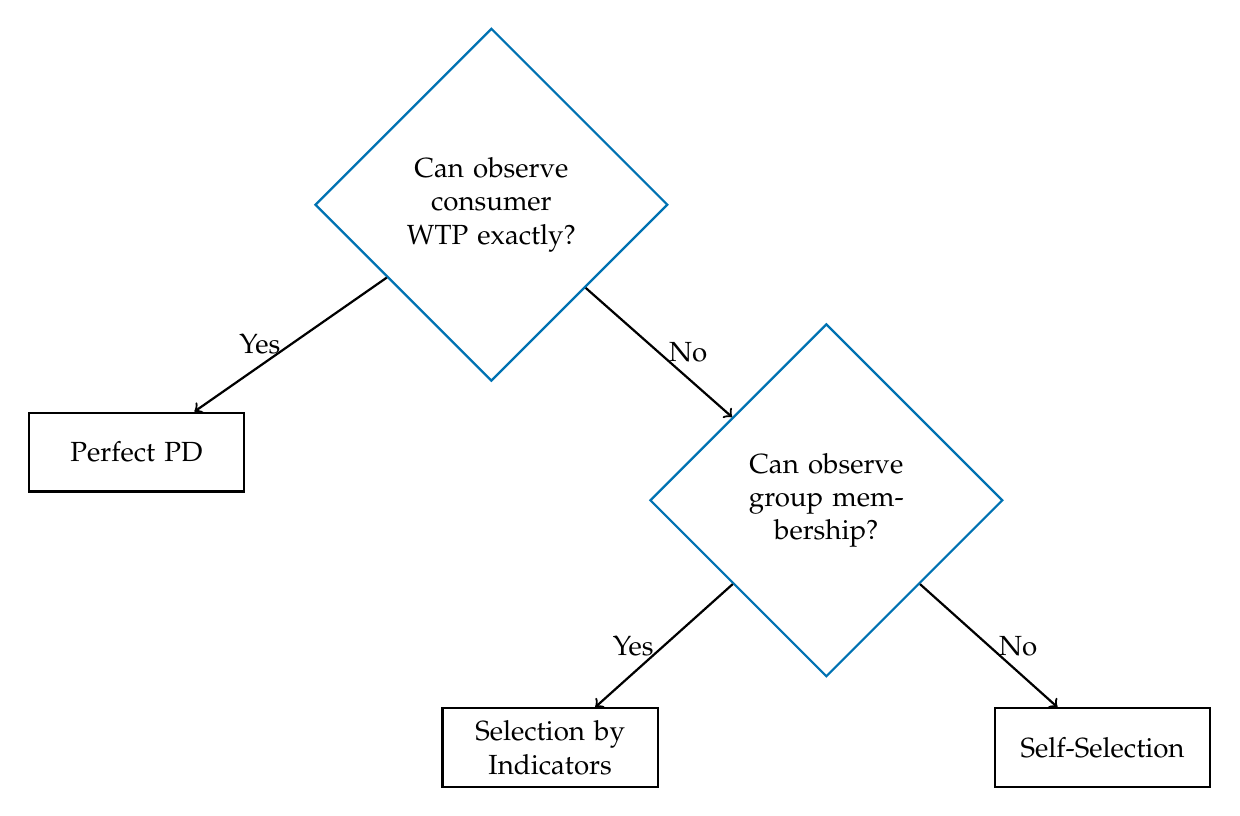
\begin{tikzpicture}[
		decision/.style={diamond, draw=blue, thick, text width=3cm, align=center, inner sep=2pt},
		block/.style={rectangle, draw=black, thick, text width=2.5cm, align=center, minimum height=1cm},
		arrow/.style={->, thick}
	]
		\node[decision] (q1) {Can observe consumer WTP exactly?};
		\node[block, below left=1.5cm and 2cm of q1] (perfect) {Perfect PD};
		\node[decision, below right=1.5cm and 2cm of q1] (q2) {Can observe group membership?};
		\node[block, below left=1.5cm and 1cm of q2] (indicator) {Selection by Indicators};
		\node[block, below right=1.5cm and 1cm of q2] (self) {Self-Selection};

		\draw[arrow] (q1) -- node[left] {Yes} (perfect);
		\draw[arrow] (q1) -- node[right] {No} (q2);
		\draw[arrow] (q2) -- node[left] {Yes} (indicator);
		\draw[arrow] (q2) -- node[right] {No} (self);
	\end{tikzpicture}
	\end{center}
	\vspace{5pt}
	\begin{wideitemize}
		\item Self-selection: design menu so consumers reveal their type
	\end{wideitemize}
\end{frame}

\begin{frame}{Midterm preparation checklist}
	\begin{wideenumerate}
		\item[$\square$] \textbf{Formulas:} Logit shares, Berry inversion, elasticities, log-sum
		\item[$\square$] \textbf{Derivations:} Can derive $MR = MC$, Lerner from FOC
		\item[$\square$] \textbf{Identification:} Why OLS biased, what makes good IVs
		\item[$\square$] \textbf{IIA:} Red bus/blue bus, when it matters
		\item[$\square$] \textbf{Pricing:} Lerner, inverse elasticity rule for segments
		\item[$\square$] \textbf{Two-part tariffs:} $p = MC$, $F = CS$; heterogeneity tradeoff
		\item[$\square$] \textbf{Self-selection:} IC/IR constraints, which binds for whom
		\item[$\square$] \textbf{Practice:} Worked through HW1 and practice exam
	\end{wideenumerate}
\end{frame}

%%%%%%%%%%%%%%%%%%%%%%%%%%%%%%%%%%%%%%%%%%%%%%%%%%%%%%%%%%%%%
% EXAM LOGISTICS
%%%%%%%%%%%%%%%%%%%%%%%%%%%%%%%%%%%%%%%%%%%%%%%%%%%%%%%%%%%%%

\begin{frame}{Plan}
  \begin{wideenumerate}
    \item Review: Demand estimation
    \item Practice problems: Demand
    \item Review: Pricing and price discrimination
    \item Practice problems: Pricing
    \item \textbf{Exam logistics}
  \end{wideenumerate}
\end{frame}

\begin{frame}{Exam format reminder}
	\begin{wideitemize}
		\item \textbf{Date:} Monday, Feb 9 (Lecture 7)
		\item \textbf{Duration:} 80 minutes
		\item \textbf{Allowed:} Calculator + two-sided cheat sheet
		\item \textbf{Coverage:}
		\begin{wideitemize}
			\vspace{5pt}
			\item Demand: logit, Berry inversion, elasticities, IVs, IIA, CS
			\item Pricing: monopoly, Lerner index, price discrimination
			\item Two-part tariffs, self-selection (IC/IR)
		\end{wideitemize}
		\item \textbf{Format:} Mix of T/F/NEI, short answer, and problems
	\end{wideitemize}
\end{frame}

\begin{frame}{What to put on your cheat sheet}
	\begin{wideitemize}
		\item \textbf{Key formulas:}
		\begin{wideitemize}
			\vspace{5pt}
			\item Logit share, Berry inversion
			\item Own and cross elasticities
			\item Log-sum formula for CS
			\item Lerner index
			\item Two-part tariff optimal conditions
		\end{wideitemize}
		\item \textbf{Worked examples:} Similar to practice problems
		\item \textbf{Key intuitions:}
		\begin{wideitemize}
			\vspace{5pt}
			\item Why price endogeneity biases $\alpha$ toward zero
			\item Why IC binds for high type, IR for low type
		\end{wideitemize}
	\end{wideitemize}
\end{frame}

%%%%%%%%%%%%%%%%%%%%%%%%%%%%%%%%%%%%%%%%%%%%%%%%%%%%%%%%%%%%%
% KEY POINTS
%%%%%%%%%%%%%%%%%%%%%%%%%%%%%%%%%%%%%%%%%%%%%%%%%%%%%%%%%%%%%

\begin{frame}{Key Points}
	\vspace{11pt}
	\begin{wideenumerate}
		\item \textbf{Logit:} $s_j = \exp(\delta_j)/[1 + \Sigma\exp(\delta_k)]$
		\item \textbf{Berry inversion:} $\ln(s_j) - \ln(s_0) = \delta_j$
		\item \textbf{Elasticities:} Own: $\alpha p_j(1-s_j)$; Cross: $-\alpha p_k s_k$
		\item \textbf{IVs needed} because $E[p_j \xi_j] \neq 0$; bias toward zero
		\item \textbf{Lerner:} $L = (p-MC)/p = 1/|\varepsilon|$
		\item \textbf{Selection by indicators:} Higher price in inelastic market
		\item \textbf{Two-part tariff:} $p = MC$, $F = CS$
		\item \textbf{Self-selection:} IC binds for high type, IR for low type
	\end{wideenumerate}
\end{frame}

\begin{frame}{Good luck on the midterm!}
	\begin{wideitemize}
		\item \textbf{Office hours:} [TBD]
		\item \textbf{Practice exam:} Posted on course website
		\item Questions?
	\end{wideitemize}
\end{frame}

%%%%%%%%%%%%%%%%%%%%%%%%%%%%%%%%%%%%%%%%%%%%%%%%%%%%%%%%%%%%%
% PREVIEW OF PART 2 (NOT ON MIDTERM)
%%%%%%%%%%%%%%%%%%%%%%%%%%%%%%%%%%%%%%%%%%%%%%%%%%%%%%%%%%%%%

\begin{frame}{What's coming after the midterm}
	\begin{wideitemize}
		\item \textbf{Part 2: Models of Competition}
		\begin{wideitemize}
			\vspace{5pt}
			\item Oligopoly models (Cournot, Bertrand, Hotelling)
			\item Entry and entry deterrence
			\item Mergers and merger simulation
			\item Vertical relationships
			\item Collusion
		\end{wideitemize}
		\item \textbf{Connection to Part 1:} We'll use demand estimation to analyze competition
		\item \textbf{HW2:} Merger simulation using your demand estimates
	\end{wideitemize}
\end{frame}

\begin{frame}{Refresher: Cournot competition}
	\begin{wideitemize}
		\item You covered this in ECN 532 (Hector's class)
		\item \textbf{Setup:} $n$ firms choose quantities simultaneously
		\item \textbf{Key result:} Lerner index in Cournot equilibrium
		\begin{align*}
			L_i = \frac{P - MC}{P} = \frac{s_i}{|\varepsilon|}
		\end{align*}
		\item \textbf{Interpretation:}
		\begin{wideitemize}
			\vspace{5pt}
			\item Markup depends on market share $s_i$
			\item More elastic demand $\rightarrow$ lower markup
		\end{wideitemize}
		\item This connects oligopoly theory to our demand estimation!
	\end{wideitemize}
\end{frame}

\begin{frame}{Refresher: Bertrand competition}
	\begin{wideitemize}
		\item \textbf{Setup:} Firms choose prices simultaneously (homogeneous goods)
		\item \textbf{Key result:} $P = MC$ (even with just 2 firms!)
		\item \textbf{The Bertrand Paradox:}
		\begin{wideitemize}
			\vspace{5pt}
			\item Two firms enough for perfectly competitive outcome
			\item Seems unrealistic---most oligopolies have positive profits
		\end{wideitemize}
		\item \textbf{Escaping the paradox:}
		\begin{wideitemize}
			\vspace{5pt}
			\item Product differentiation (Hotelling)
			\item Capacity constraints
			\item Repeated interaction (collusion)
		\end{wideitemize}
	\end{wideitemize}
\end{frame}

\begin{frame}{Why this matters for Part 2}
	\begin{wideitemize}
		\item \textbf{Mergers:} Understanding how firms compete tells us merger effects
		\begin{wideitemize}
			\vspace{5pt}
			\item Cournot merger: internalize quantity competition
			\item Bertrand merger: internalize price competition
		\end{wideitemize}
		\item \textbf{Entry:} Market structure determines profitability
		\item \textbf{Policy:} Antitrust authorities use these models
		\item \textbf{HW2 preview:} You'll simulate a merger using demand estimates
	\end{wideitemize}
	\vspace{10pt}
	\centering
	\textit{We'll cover this in detail after the midterm!}
\end{frame}

\end{document}
